В библиотеке \textbf{numpy.fft} есть функция \textbf{fft}, которая реализует быстрое преобразование Фурье. Задается она, согласно документации, следующим образом:
\begin{equation}
    F(k) = \sum_{m=0}^{N-1} f(m) e^{-2\pi i \dfrac{k m}{N}} 
\end{equation}
И обратное преобразование Фурье \textbf{ifft}: 
\begin{equation}
    f(m) = \frac{1}{N} \sum_{k=0}^{N-1} F(k) e^{2\pi i \dfrac{k m}{N}}
\end{equation}
Для того, чтобы сделать это преобразование унитарным, необходимо 
умножить результат прямого преобразования на $\dfrac{1}{\sqrt{N}}$, а результат обратного преобразования на $\sqrt{N}$ или добавить параметр \textbf{norm='ortho'}. Дальше будем считать, что это сделано.

\subsection{Восстановление функции из ее образа}
\def\steps{10000}
Посмотрим на то, как будет выглядеть восстановленная из образа функции при использовании \texttt{ifft} на рисунке \ref{fig:\steps_ifft_cmp}.
\begin{figure}[ht!]
    \centering
    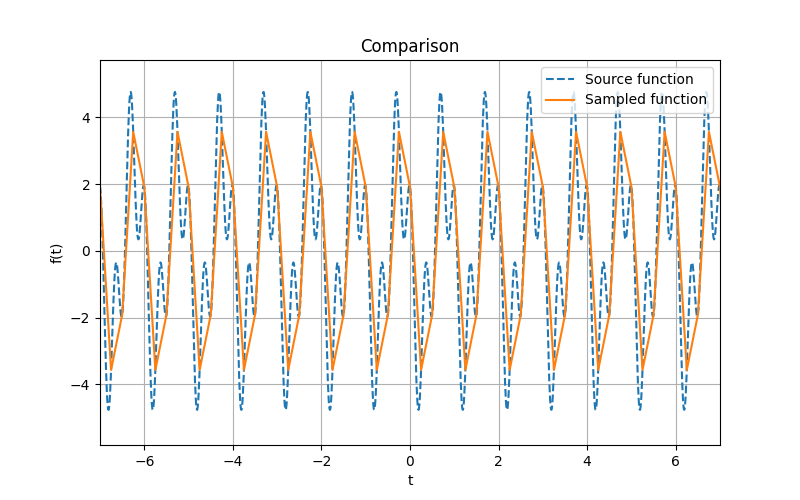
\includegraphics[width=\textwidth]{plots/fft_\steps/cmp_func}
    \caption{Сравнение исходной и восстановленной функции (разбиение на $\steps$ точек)}
    \label{fig:\steps_ifft_cmp}
\end{figure}

На рисунке \ref{fig:\steps_ifft_cmp} видно, что исходная и восстановленная функции совпадают. 
Посмотрим на график разности исходной и восстановленной функции на рисунке \ref{fig:\steps_ifft_error}.
\begin{figure}[ht!]
    \centering
    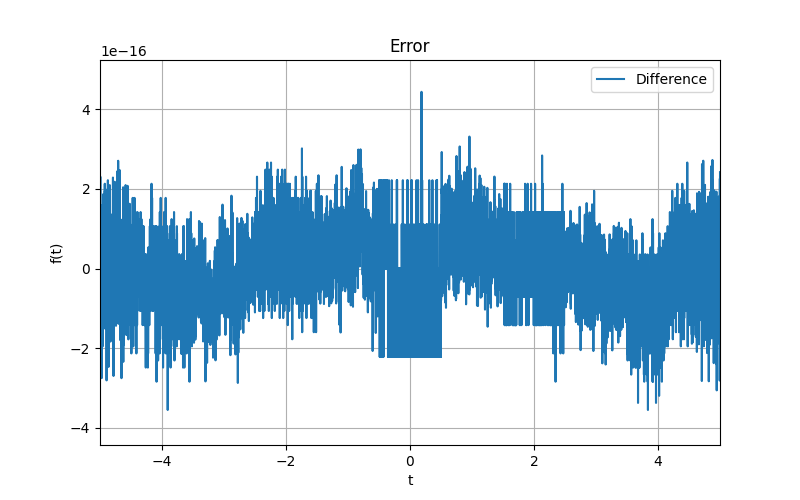
\includegraphics[width=\textwidth]{plots/fft_\steps/error}
    \caption{Разность исходной и восстановленной функции (разбиение на $\steps$ точек)}
    \label{fig:\steps_ifft_error}
\end{figure}

Видно, что ошибка по модулю не превышает $4 \cdot 10^{-16}$, что говорит о том, что восстановленная функция практически идеально совпадает с исходной.
При этом скорость работы алгоритма быстрого преобразования Фурье значительно выше, чем обычного преобразования Фурье.

\subsection{Нахождение образа}

Для начала, попробуем построить график образа функции, который получился в результате применения \texttt{fft} на рисунке \ref{fig:\steps_fft_image}.
\begin{figure}[ht!]
    \centering
    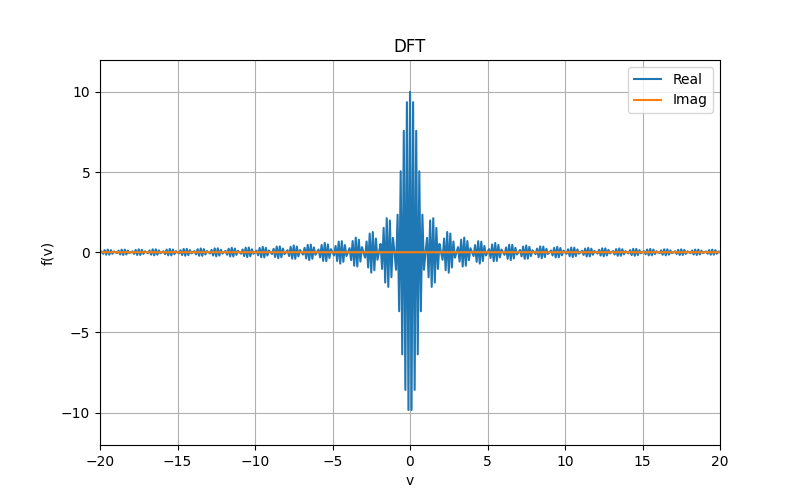
\includegraphics[width=\textwidth]{plots/fft_\steps/dft_image}
    \caption{Образ функции (разбиение на $\steps$ точек)}
    \label{fig:\steps_fft_image}
\end{figure}

Видно, что получился график вовсе не похож на истинный образ функции. 

Теперь рассмотрим \textit{правильный} способ нахождения образа функции через DFT. 
Для этого рассмотрим преобразование Фурье (см. формулу \eqref{eq:fourier}) и попробуем дискретизировать его (см. формулу \eqref{eq:dis_fourier} и \eqref{eq:dis_fourier2}) введя параметры 
$t_d = m\Delta t + t_0$, $v_d = k\Delta v$, где $t_d,~v_d$ -- дискретное время и частота соответственно. $\Delta t \Delta v = \frac{1}{N}$
\begin{equation}
    \hat{f}(v) = \frac{1}{\sqrt{2\pi}}\int_{-\infty}^{\infty} f(t) e^{-2\pi i v t} dt 
    \label{eq:fourier}
\end{equation}
\begin{multline}
    \hat{f}(v) = \frac{1}{\sqrt{N}}\sum_{m=0}^{N-1} f(t_d) e^{-2\pi i v} \Delta t = \frac{1}{\sqrt{N}}\sum_{m=0}^{N-1} f(m\Delta t + t_0) e^{-2\pi i v( m\Delta t + t_0)} \Delta t = \\
    \frac{1}{\sqrt{N}}\sum_{m=0}^{N-1} f(m\Delta t + t_0) e^{-2\pi i m v \Delta t -2\pi i v t_0} \Delta t =  \Delta te^ {-2\pi i v t_0} \frac{1}{\sqrt{N}}\sum_{m=0}^{N-1} f(m\Delta t + t_0) e^{-2\pi i v m \Delta t} 
    \label{eq:dis_fourier} 
\end{multline}
\begin{equation}
    \hat{f}(v_d) = \Delta te^ {-2\pi i v_d t_0}\frac{1}{\sqrt{N}} \sum_{m=0}^{N-1} f(m\Delta t + t_0) e^{-2\pi i km \Delta v \Delta t} = \Delta te^ {-2\pi i v_d t_0}\frac{1}{\sqrt{N}} \sum_{m=0}^{N-1} f(t_d) e^{-2\pi i km / N} 
    \label{eq:dis_fourier2} 
\end{equation}
Заметим, что правая часть произведения является DFT образом функции. Таким образом, получим: 
\begin{equation}
    \hat{f}(v_d) = \Delta te^ {-2\pi i v_d t_0} \frac{1}{\sqrt{N}}\sum_{m=0}^{N-1} f(t_d) e^{-2\pi i km / N} = \Delta te^ {-2\pi i v_d t_0} \cdot F(t_d)
    \label{eq:dis_fourier3}
\end{equation}

Левую часть произведения можно назвать фазовым коэффициентом, а правая часть -- DFT образом функции. Получается, что для того, чтобы получить 
образ функции из DFT, необходимо умножить его на фазовый коэффициент. 

Полученный образ приведен на рисунке \ref{fig:\steps_dft_cont_image}. Сравнительный график образа функции, полученного через DFT и аналитически на рисунке \ref{fig:\steps_cmp_cont_image}.
\begin{figure}
    \centering
    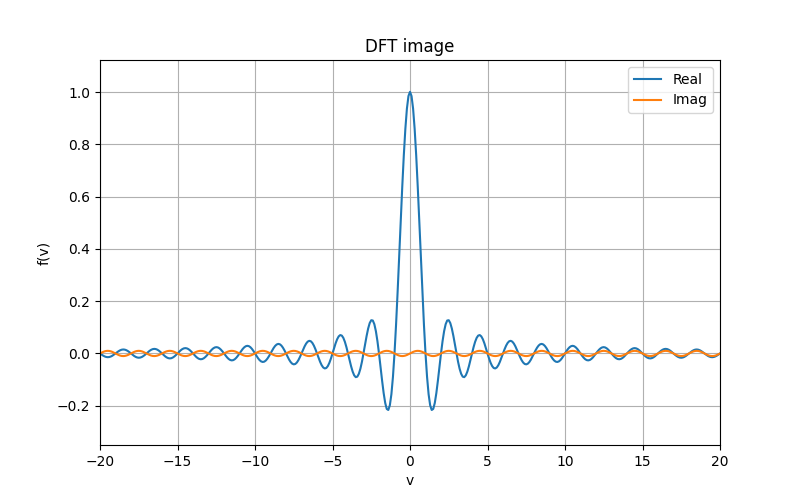
\includegraphics[width=\textwidth]{plots/fft_\steps/dft_cont_image}
    \caption{Образ функции, полученный через DFT (разбиение на $\steps$ точек)}
    \label{fig:\steps_dft_cont_image}
\end{figure}
\begin{figure}
    \centering
    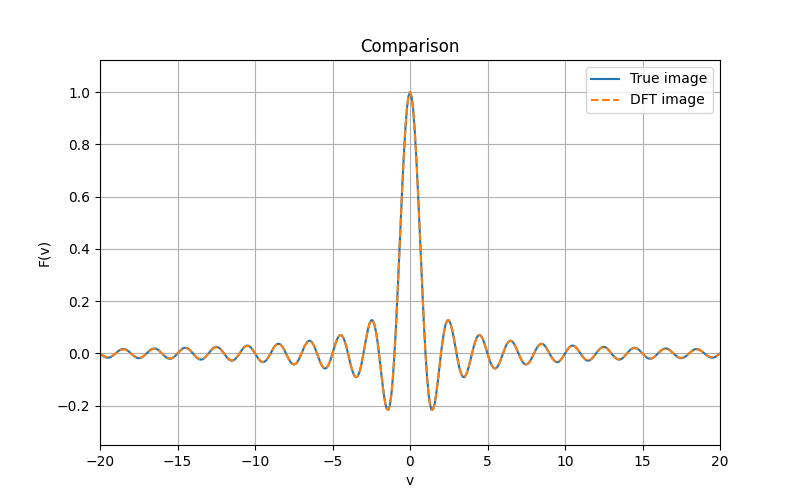
\includegraphics[width=\textwidth]{plots/fft_\steps/cmp_cont_image}
    \caption{Сравнение аналитического и DFT образа функции (разбиение на $\steps$ точек)}
    \label{fig:\steps_cmp_cont_image}
\end{figure}

Видно, что графики совпадают. Таким образом, можно сделать вывод о том, что данное преобразование работает корректно. 

Для применения обратного преобразования так же рассмотрим формулу \eqref{eq:ifourier} и преобразуем ее:
\begin{equation}
    f(t) = \frac{1}{\sqrt{2\pi}}\int_{-\infty}^{\infty} \hat{f}(v) e^{2\pi i v t} dv 
    \label{eq:ifourier}
\end{equation}
\begin{equation}
    f(t_d) = \frac{1}{\sqrt{N}} \sum_{m = 0}^{N - 1} \hat{f}(v_d) e^{2\pi i k\Delta v m\Delta t } \Delta v = \Delta v F(v_d) 
\end{equation}

Посмотрим на график восстановленной из образа функции на рисунке \ref{fig:\steps_num_restored_cont}.
\begin{figure}[ht!]
    \centering
    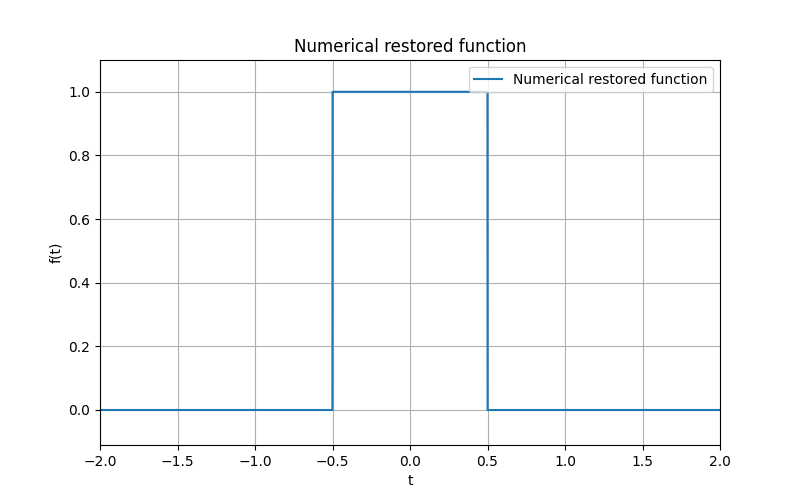
\includegraphics[width=\textwidth]{plots/fft_\steps/num_restored_cont}
    \caption{Восстановленная функция из образа (разбиение на $\steps$ точек)}
    \label{fig:\steps_num_restored_cont}
\end{figure}

Видим, что функция восстановлена верно.